%----------------------------------------------------------------------------------------
%	SLIDE 6.
%----------------------------------------------------------------------------------------
\begin{frame}
\frametitle{De még sok más is...}

\begin{block}{Példák párhuzamosítható problémákra}
	\begin{columns}
		\column{0.5\linewidth}
		\begin{itemize}
			\item Monte--Carlo-szimulációk
			\item Numerikus integrálás
			\item Machine learning algoritmusok (pl. random forest)
			\item[] $\qquad \vdots$
		\end{itemize}
		
		\column{0.5\linewidth}
		\begin{itemize}
			\item Számítógépes vizualizációk és modellezés
			\item Képfeldolgozási problémák
			\item Diszkrét Fourier-transzformáció
			\item[] $\qquad \vdots$
		\end{itemize}
	\end{columns}
\end{block}

\begin{columns}
	\column{0.3\linewidth}
	\begin{figure}
		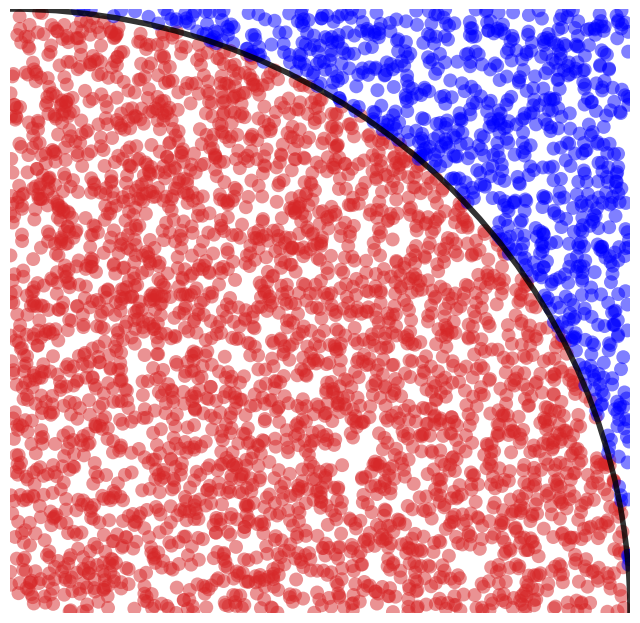
\includegraphics[width=\textwidth]{img/monte_carlo.png}
	\end{figure}	
	
	\column{0.4\linewidth}
	\begin{figure}
		
\includegraphics[width=\textwidth]{img/rfr-xgb.jpg}
	\end{figure}	
	
	\column{0.3\linewidth}
	\begin{figure}
		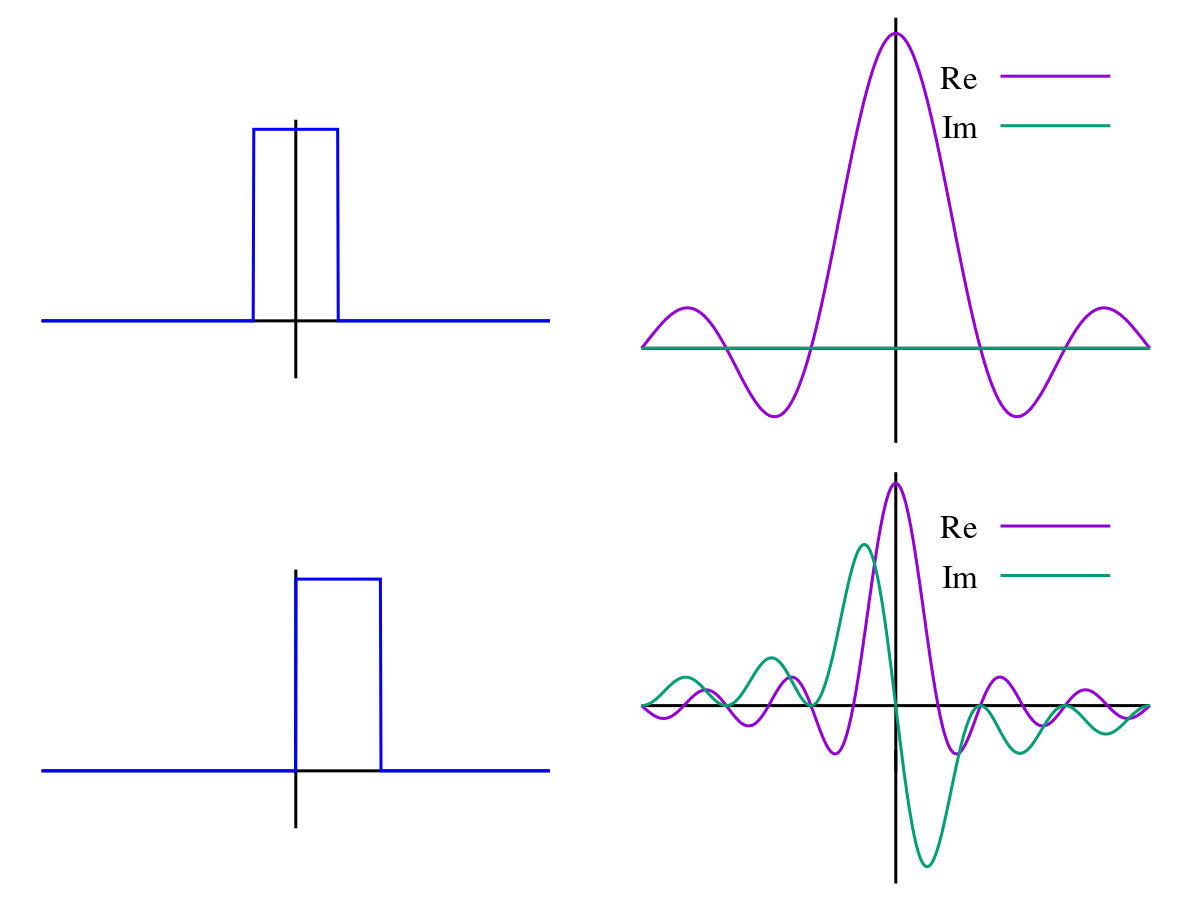
\includegraphics[width=\textwidth]{img/fourier.png}
	\end{figure}	
\end{columns}

\end{frame}